
%%%%%%%%%%%%%%%%%%%%%%%%%%%%%%%%%%%%%%%%%
% Short Sectioned Assignment LaTeX Template Version 1.0 (5/5/12)
% This template has been downloaded from: http://www.LaTeXTemplates.com
% Original author:  Frits Wenneker (http://www.howtotex.com)
% License: CC BY-NC-SA 3.0 (http://creativecommons.org/licenses/by-nc-sa/3.0/)
%%%%%%%%%%%%%%%%%%%%%%%%%%%%%%%%%%%%%%%%%

%----------------------------------------------------------------------------------------
%	PACKAGES AND OTHER DOCUMENT CONFIGURATIONS
%----------------------------------------------------------------------------------------

\documentclass[paper=a4, fontsize=11pt]{scrartcl} % A4 paper and 11pt font size

% ---- Entrada y salida de texto -----

\usepackage[T1]{fontenc} % Use 8-bit encoding that has 256 glyphs
\usepackage[utf8]{inputenc}
%\usepackage{fourier} % Use the Adobe Utopia font for the document - comment this line to return to the LaTeX default
\usepackage{listings}
\usepackage{xcolor}
\lstset { %
	language=C++,
	frame=tb, % draw a frame at the top and bottom of the code block
	tabsize=4, % tab space width
	showstringspaces=false, % don't mark spaces in strings
	numbers=left, % display line numbers on the left
	commentstyle=\color{green}, % comment color
	keywordstyle=\color{blue}, % keyword color
	stringstyle=\color{red} % string color
}


% ---- Idioma --------

\usepackage[spanish, es-tabla]{babel} % Selecciona el español para palabras introducidas automáticamente, p.ej. "septiembre" en la fecha y especifica que se use la palabra Tabla en vez de Cuadro

% ---- Otros paquetes ----

\usepackage{url} % ,href} %para incluir URLs e hipervínculos dentro del texto (aunque hay que instalar href)
\usepackage{amsmath,amsfonts,amsthm} % Math packages
%\usepackage{graphics,graphicx, floatrow} %para incluir imágenes y notas en las imágenes
\usepackage{graphics,graphicx, float} %para incluir imágenes y colocarlas

% Para hacer tablas comlejas
\usepackage{multirow}
\usepackage{threeparttable}
\usepackage{booktabs}

%\usepackage{sectsty} % Allows customizing section commands
%\allsectionsfont{\centering \normalfont\scshape} % Make all sections centered, the default font and small caps

\usepackage{fancyhdr} % Custom headers and footers
\pagestyle{fancyplain} % Makes all pages in the document conform to the custom headers and footers
\fancyhead{} % No page header - if you want one, create it in the same way as the footers below
\fancyfoot[L]{} % Empty left footer
\fancyfoot[C]{} % Empty center footer
\fancyfoot[R]{\thepage} % Page numbering for right footer
\renewcommand{\headrulewidth}{0pt} % Remove header underlines
\renewcommand{\footrulewidth}{0pt} % Remove footer underlines
\setlength{\headheight}{13.6pt} % Customize the height of the header

\numberwithin{equation}{section} % Number equations within sections (i.e. 1.1, 1.2, 2.1, 2.2 instead of 1, 2, 3, 4)
\numberwithin{figure}{section} % Number figures within sections (i.e. 1.1, 1.2, 2.1, 2.2 instead of 1, 2, 3, 4)
\numberwithin{table}{section} % Number tables within sections (i.e. 1.1, 1.2, 2.1, 2.2 instead of 1, 2, 3, 4)

\setlength\parindent{0pt} % Removes all indentation from paragraphs - comment this line for an assignment with lots of text

\newcommand{\horrule}[1]{\rule{\linewidth}{#1}} % Create horizontal rule command with 1 argument of height


\graphicspath{{images/}}

%----------------------------------------------------------------------------------------
%	TÍTULO Y DATOS DEL ALUMNO
%----------------------------------------------------------------------------------------

\title{	
\normalfont \normalsize 
\textsc{\textbf{Fundamentos de Ingeniería del Software (2018-2019)} \\ Doble Grado en Ingeniería Informática Y Matemáticas \\ Universidad de Granada} \\ [25pt] % Your university, school and/or department name(s)
\horrule{0.5pt} \\[0.4cm] % Thin top horizontal rule
\huge \textbf{Práctica 3} \\ Análisis y especificación de requisitos \\ % The assignment title
\horrule{2pt} \\[0.5cm] % Thick bottom horizontal rule
}

\author{Javier Alcántara García\\ César Muñoz Reinoso \\ Sergio Cabezas González de Lara \\ Víctor García Carrera} % Nombre y apellidos

\date{\normalsize\today} % Incluye la fecha actual


%----------------------------------------------------------------------------------------
% DOCUMENTO
%----------------------------------------------------------------------------------------

\begin{document}

\maketitle % Muestra el Título

\newpage %inserta un salto de página

\tableofcontents % para generar el índice de contenidos

\newpage

\section{Contratos}
\subsection{Gestión de flota}
\begin{figure}[H]
	\centering
	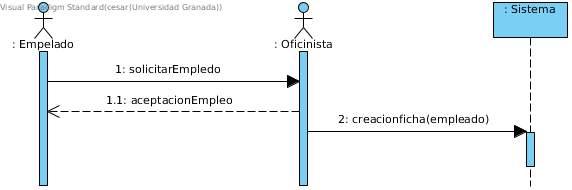
\includegraphics[width=16cm]{1}
\end{figure}
\begin{figure}[H]
	\centering
	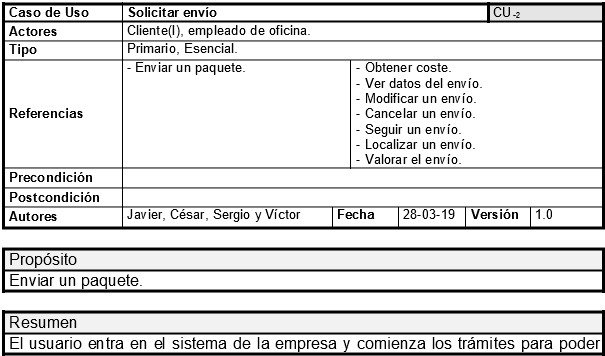
\includegraphics[width=16cm]{2}
\end{figure}
\begin{figure}[H]
	\centering
	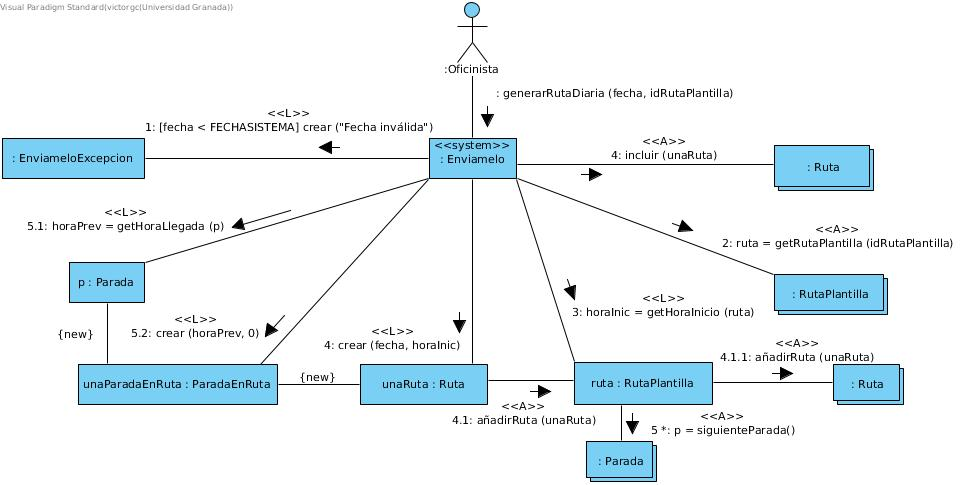
\includegraphics[width=16cm]{3}
\end{figure}
\begin{figure}[H]
	\centering
	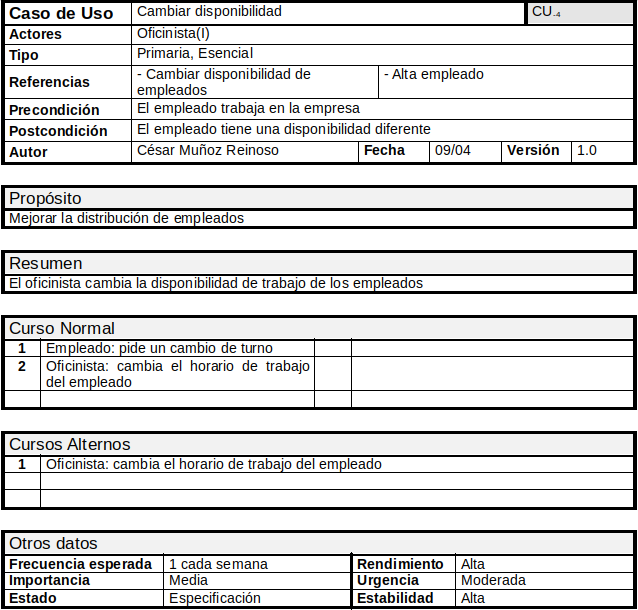
\includegraphics[width=16cm]{4}
\end{figure}
\begin{figure}[H]
	\centering
	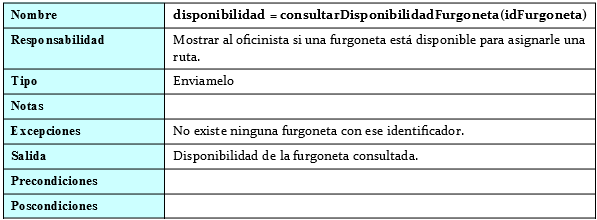
\includegraphics[width=16cm]{5}
\end{figure}
\begin{figure}[H]
	\centering
	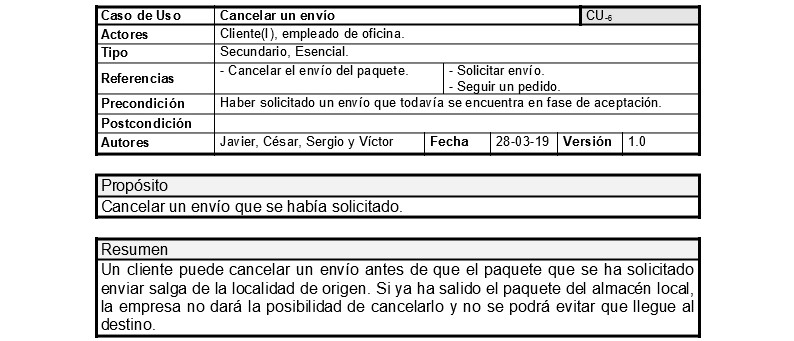
\includegraphics[width=16cm]{6}
\end{figure}
\begin{figure}[H]
	\centering
	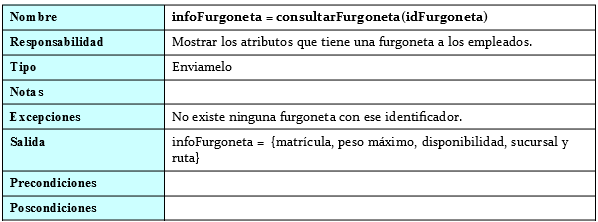
\includegraphics[width=16cm]{7}
\end{figure}
\newpage
\subsection{Gestión de Almacén}
\begin{figure}[H]
	\centering
	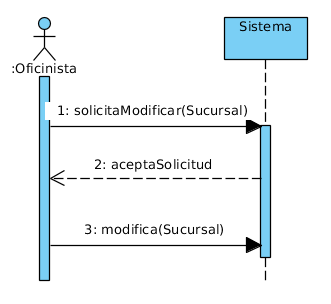
\includegraphics[width=16cm]{8}
\end{figure}
\begin{figure}[H]
	\centering
	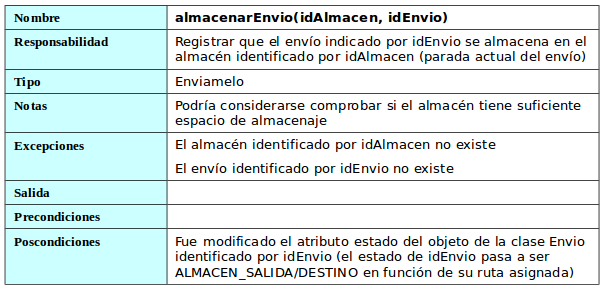
\includegraphics[width=16cm]{9}
\end{figure}
\begin{figure}[H]
	\centering
	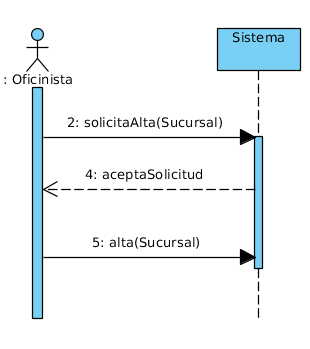
\includegraphics[width=16cm]{10}
\end{figure}
\begin{figure}[H]
	\centering
	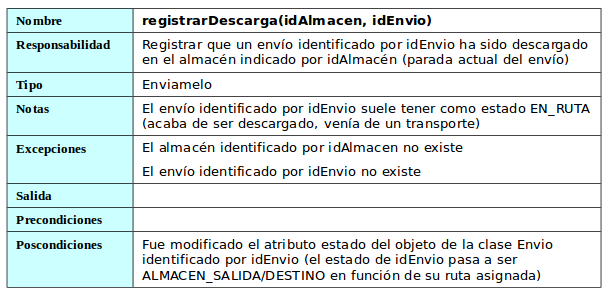
\includegraphics[width=16cm]{11}
\end{figure}
\begin{figure}[H]
	\centering
	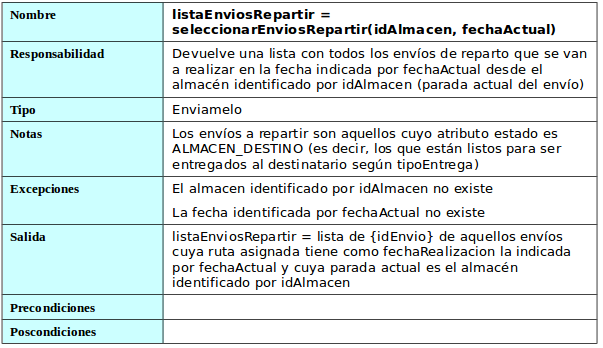
\includegraphics[width=16cm]{12}
\end{figure}
\begin{figure}[H]
	\centering
	
\includegraphics[width=16cm]{13}
\end{figure}
\begin{figure}[H]
	\centering
	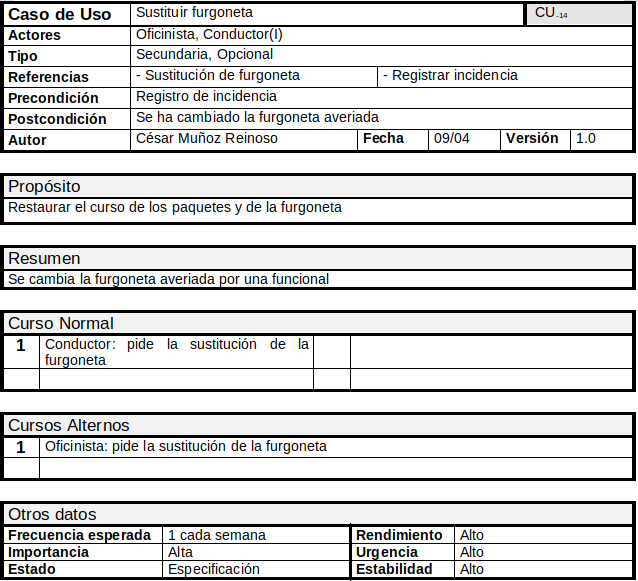
\includegraphics[width=16cm]{14}
\end{figure}
\begin{figure}[H]
	\centering
	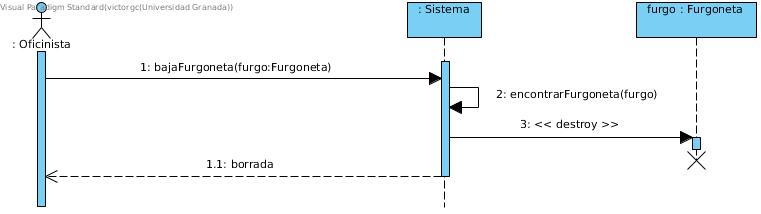
\includegraphics[width=16cm]{15}
\end{figure}
\begin{figure}[H]
	\centering
	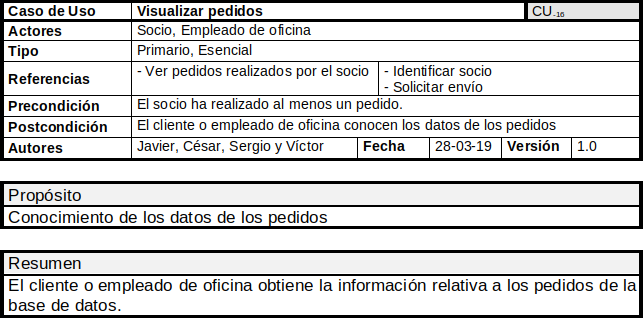
\includegraphics[width=16cm]{16}
\end{figure}
\begin{figure}[H]
	\centering
	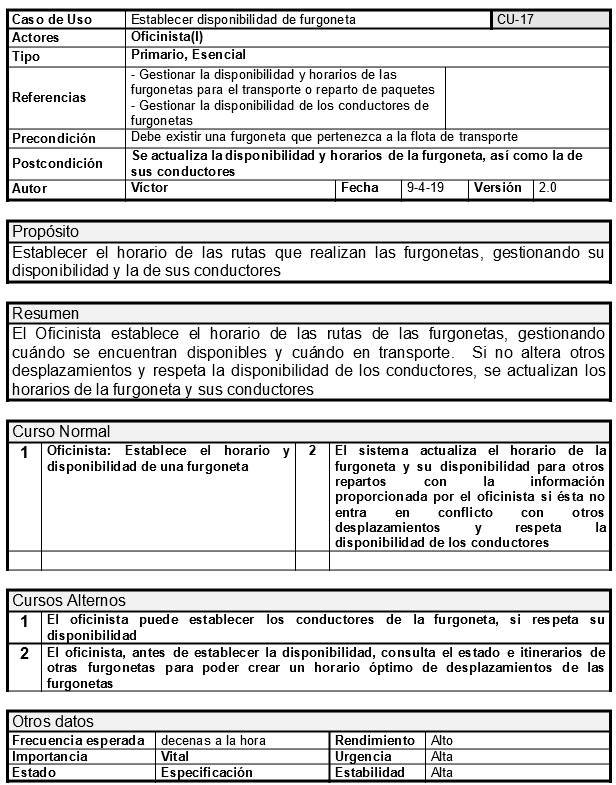
\includegraphics[width=16cm]{17}
\end{figure}
\begin{figure}[H]
	\centering
	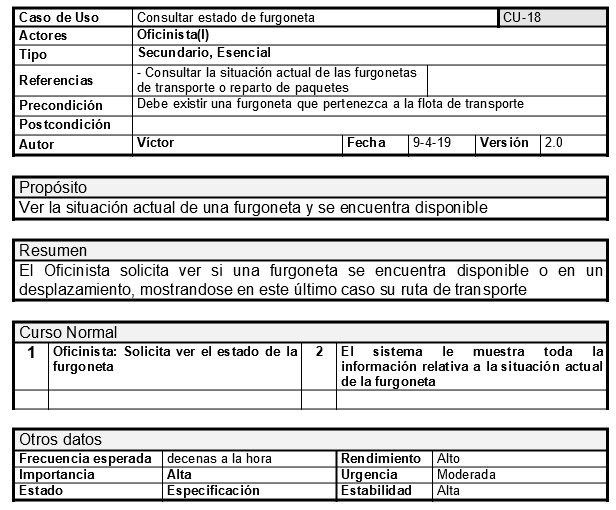
\includegraphics[width=16cm]{18}
\end{figure}
\newpage
\subsection{Gestión transporte}
\begin{figure}[H]
	\centering
	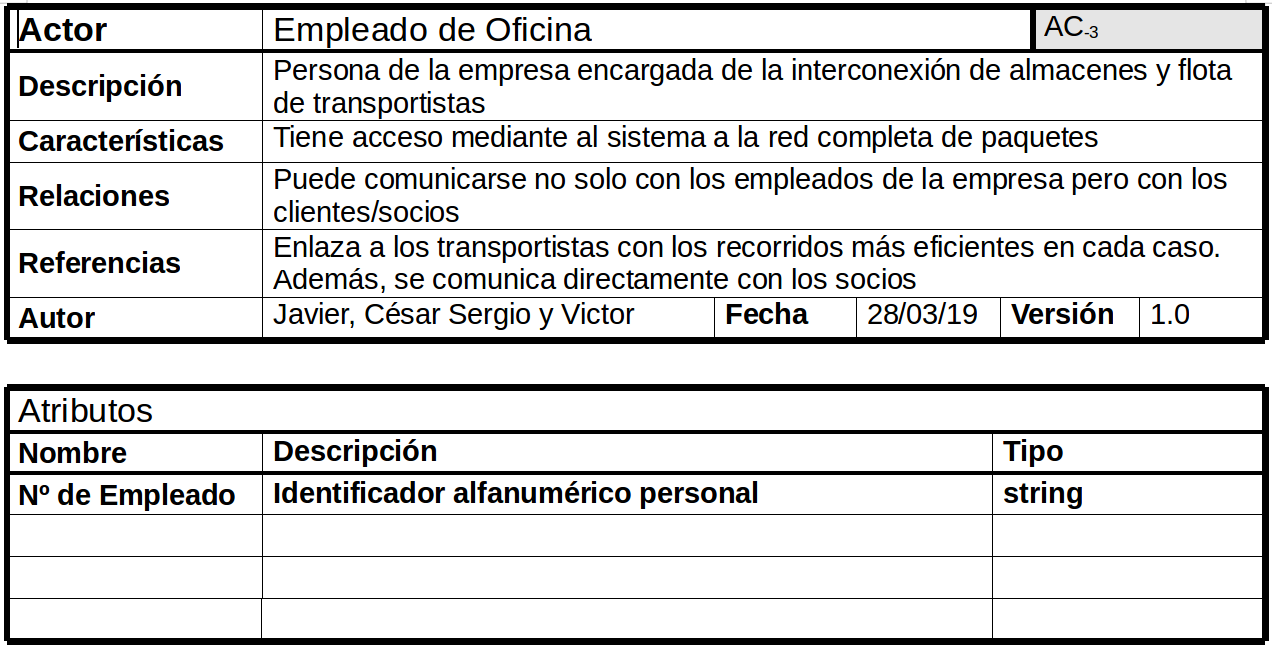
\includegraphics[width=16cm]{19}
\end{figure}
\begin{figure}[H]
	\centering
	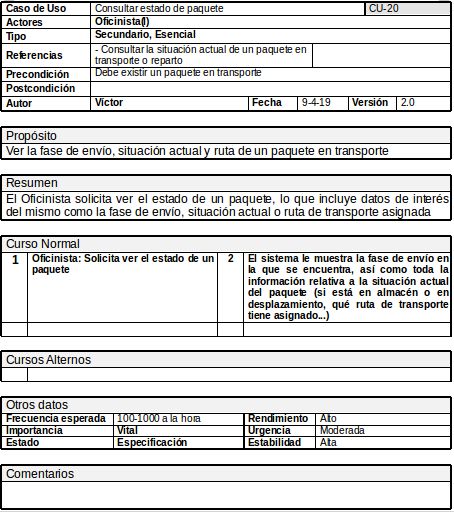
\includegraphics[width=16cm]{20}
\end{figure}
\begin{figure}[H]
	\centering
	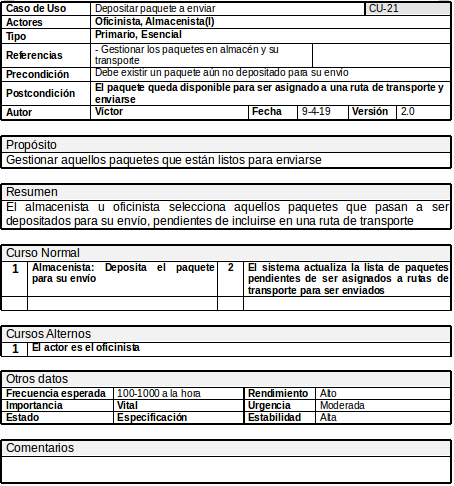
\includegraphics[width=16cm]{21}
\end{figure}
\begin{figure}[H]
	\centering
	
\includegraphics[width=16cm]{22}
\end{figure}
\begin{figure}[H]
	\centering
	
\includegraphics[width=16cm]{23}
\end{figure}
\begin{figure}[H]
	\centering
	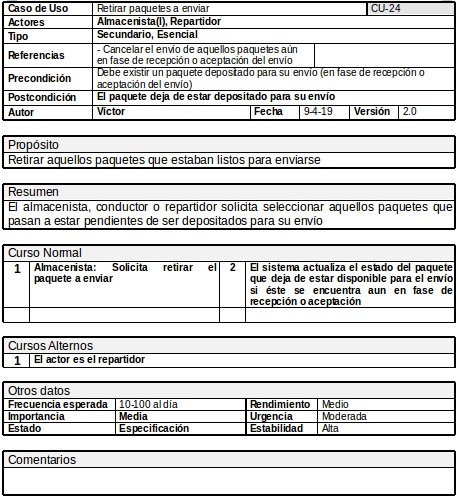
\includegraphics[width=16cm]{24}
\end{figure}
\begin{figure}[H]
	\centering
	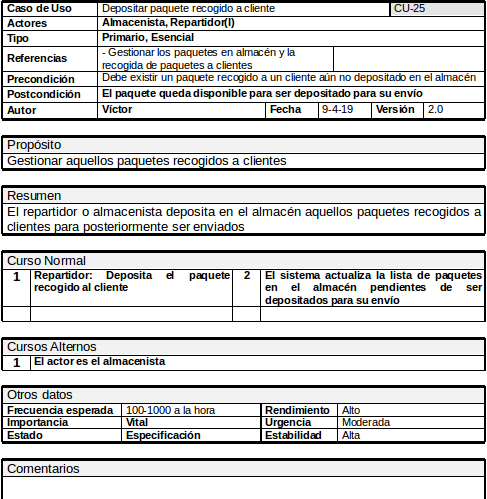
\includegraphics[width=16cm]{25}
\end{figure}
\begin{figure}[H]
	\centering
	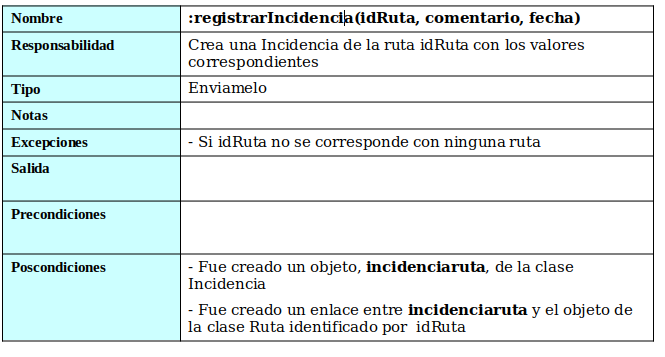
\includegraphics[width=16cm]{26}
\end{figure}
\begin{figure}[H]
	\centering
	
\includegraphics[width=16cm]{27}
\end{figure}
\begin{figure}[H]
	\centering
	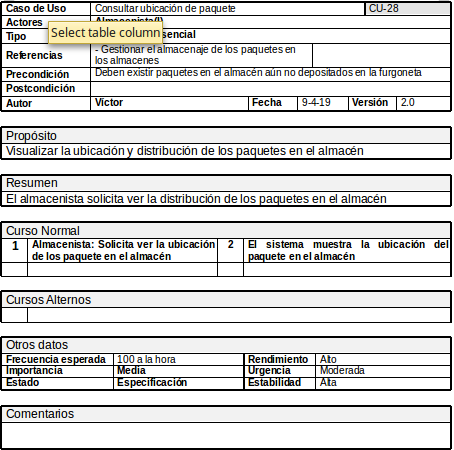
\includegraphics[width=16cm]{28}
\end{figure}
\begin{figure}[H]
	\centering
	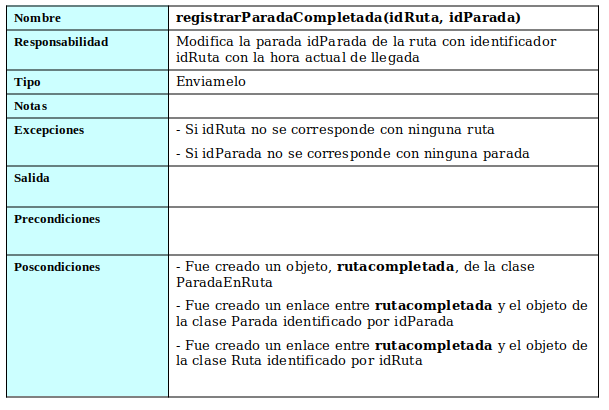
\includegraphics[width=16cm]{29}
\end{figure}
\begin{figure}[H]
	\centering
	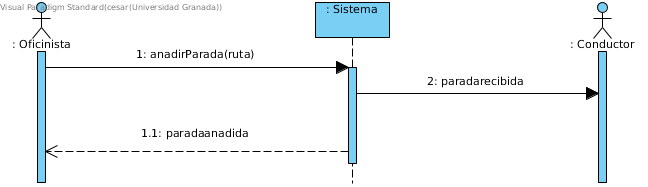
\includegraphics[width=16cm]{30}
\end{figure}
\newpage
\subsection{Atención a clientes}
\begin{figure}[H]
	\centering
	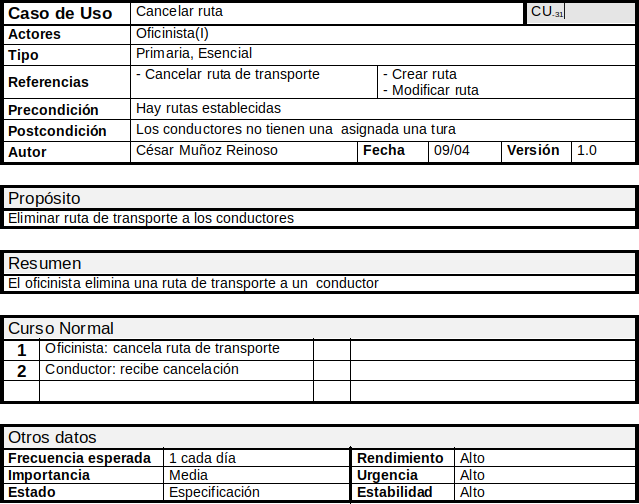
\includegraphics[width=16cm]{31}
\end{figure}
\begin{figure}[H]
	\centering
	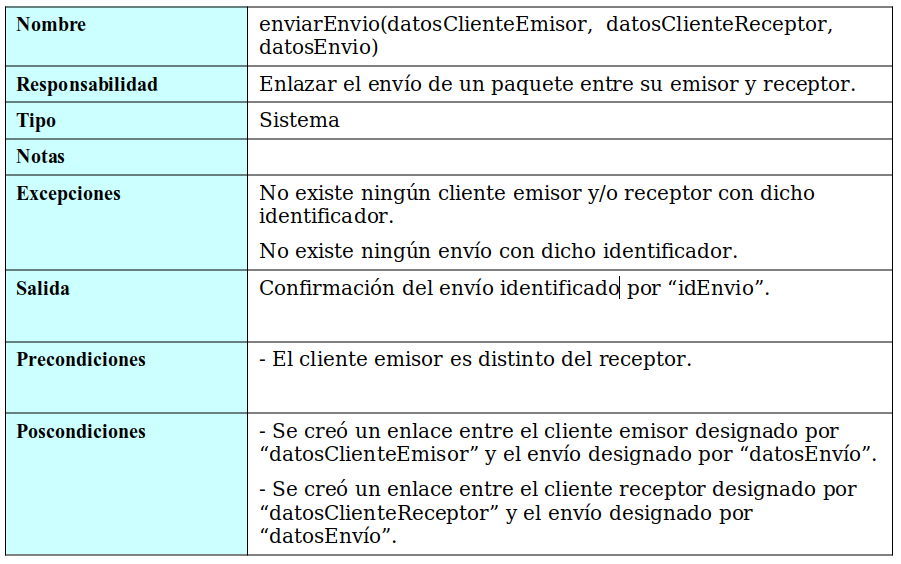
\includegraphics[width=16cm]{32}
\end{figure}
\begin{figure}[H]
	\centering
	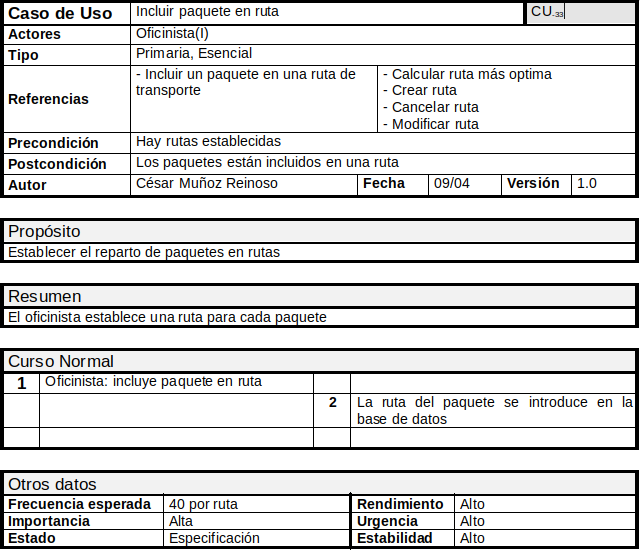
\includegraphics[width=16cm]{33}
\end{figure}
\begin{figure}[H]
	\centering
	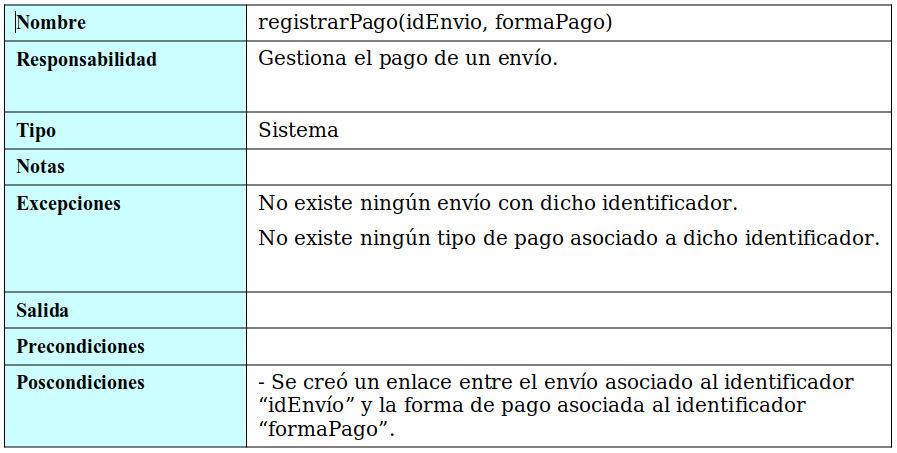
\includegraphics[width=16cm]{34}
\end{figure}
\begin{figure}[H]
	\centering
	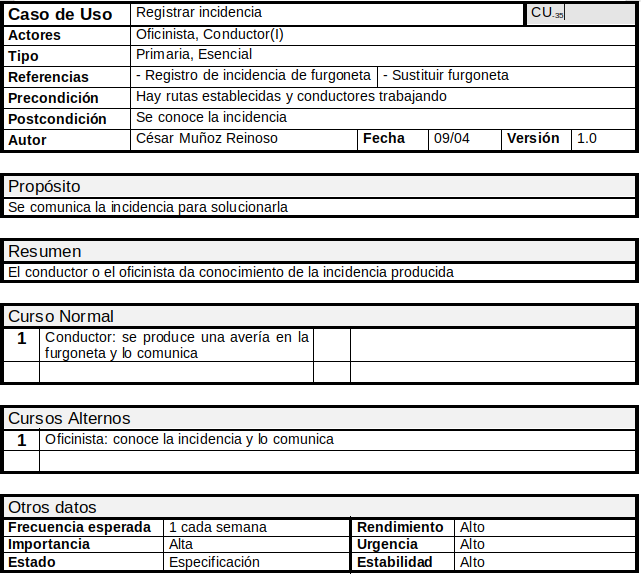
\includegraphics[width=16cm]{35}
\end{figure}
\begin{figure}[H]
	\centering
	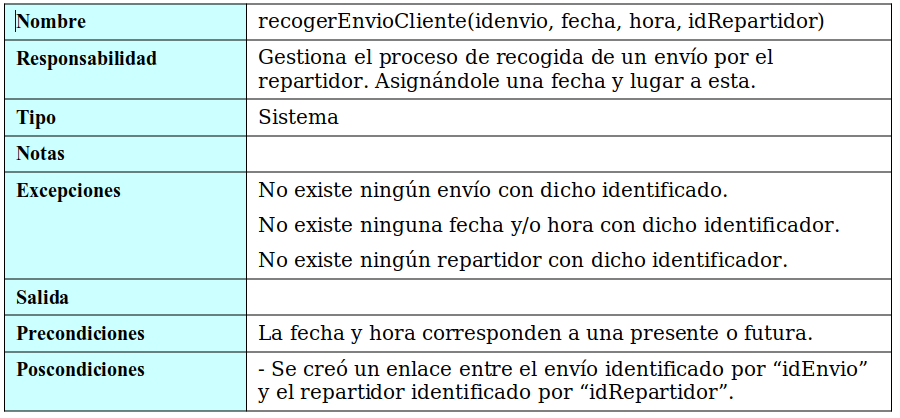
\includegraphics[width=16cm]{36}
\end{figure}
\begin{figure}[H]
	\centering
	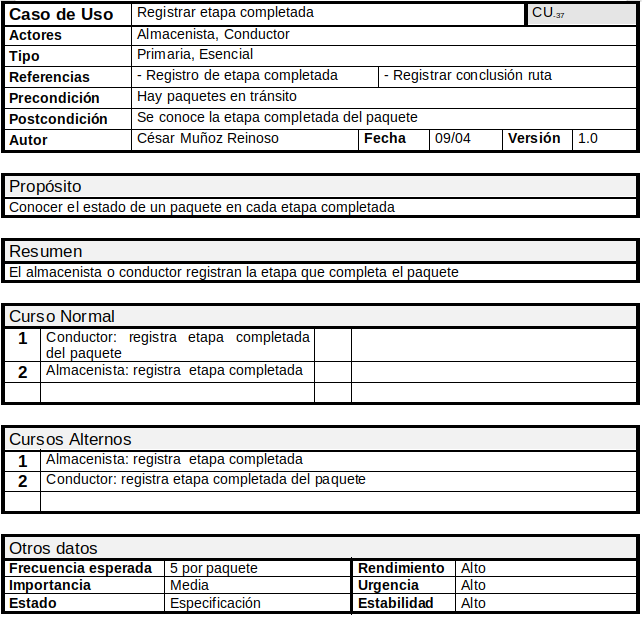
\includegraphics[width=16cm]{37}
\end{figure}

\newpage

\section{Glosario de términos}
	\begin{enumerate}
		\item \textit{Ruta de envío}: Se trata de las oficinas y almacenes por los que pasa un paquete hasta llegar al destino.
		\item \textit{Identificador de paquete}: Código que se le asigna a un paquete cuando entra al sistema de envíos de la empresa, permitiendo diferenciarlo de todos los demás y simplificar operaciones como la localización.
		\item \textit{Coste de envío}: Coste variable del servicio de envío en función del peso del paquete, dimensiones, distancia, modo de envío (certificado, urgente, etc) y condición de socio.
		\item \textit{Fase de envío}: El transporte de un paquete se divide en diversas fases: \newline - Recepción del paquete (en oficina)
		\newline - Aceptación del envío (periodo antes de que el paquete salga para su transporte para modificar el envío)
		\newline - Transporte del paquete (entre oficinas y almacenes hasta la oficina destino)
		\newline - Llegada a oficina destino
		\newline - Llegada a destino (llegada del paquete a la dirección destino)
		\item \textit{Ruta de transporte libre}: Una ruta de transporte puede estar libre o tener una furgoneta asignada.
		\item \textit{Estado de furgoneta}: Una furgoneta puede encontrarse disponible o realizando un desplazamiento, en cuyo caso incluye la ruta de transporte que está llevando a cabo.
		\item \textit{Estado de paquete}: El estado de un paquete está formado por la fase de envío en la que se encuentra, su situación y ubicación actuales y su ruta de transporte asignada.
		\item \textit{Filtro}: Herramienta externa (ej. Google Maps) que se implementa  en el sistema para comprobar si hay algún error de entrada por parte del usuario que solicita una recogida/entrega de paquete.
		\item \textit{Canal de comunicación}: Medio por el que se transmite la información sobre el envío siendo destinatario el usuario(vía e-mail o SMS).
		\item \textit{Valoraciones}: Calificación de 0 a 5 y comentarios respecto a el servicio prestado por parte de la empresa.
		\item \textit{Almacenista}: Empleado encargado de la gestión de paquetes dentro del almacén.
		\item \textit{Empleado}: Trabajador de la empresa de transportes.
		\item \textit{Oficinista}: Empleado encargado de los tramites administrativos dentro de la empresa así como la gestión general de paquetes.
		\item \textit{Almacenista}: Empleado encargado de la distribución de paquetes en los almacenes.
		\item \textit{Conductor}: Empleado encargado del transporte de paquetes entre almacenes.	
		\item \textit{Repartidor}: Empleado encargado de la recogida y entrega de paquetes entre clientes y almacenes.
		\item \textit{Sucursal}: Oficina o almacén de la empresa.
		\item \textit{Almacén}: Edificio donde se guardan y almacenan los paquetes durante su envío hasta el destino.
		\item \textit{Área personal}: Sitio web al que se accede un cliente registrado tras identificarse y con el que puede acceder a los servicios que ofrece la empresa.
 	\end{enumerate}
\newpage
%------------------------------------------------

\end{document}
